\documentclass{article}
\usepackage{soul}
\usepackage{xcolor}  % 需要这个包来改变颜色
\sethlcolor{pink}  % 设置highlight的颜色为红色
\usepackage{amsmath}
\usepackage{amssymb}
\usepackage{cancel}
\usepackage{graphicx}
\usepackage{tikz}


\title{MATH1023/MATH1062 Calculas}
\author{Usyd Mingyuan Ba}
\date{\today}

\begin{document}

\maketitle

\section{Week1}
  \subsection{Differential Equation}
  \begin{enumerate}

    \item \textbf{Differential Equation(DE)}: A differential equation (DE) is a mathmatical equation that relates some \hl{function with its derivatives}

    \item \textbf{Order}: The order of a differential equation equals to a \hl{highest derivative} occuring in it.
      \begin{itemize}
        \item $\frac{dy}{dx} = -ky$ has order \hl{$1$}
        \item $\frac{dy}{dx} = y^{18} + \frac{d^5y}{dx^2}y + x^2$ has order \hl{5}
      \end{itemize}

    \item \textbf{Standard Form}: The standard form of a \hl{first-order differential equation} is 
      \begin{center}
        $\frac{dy}{dx} = f(x,y)$
      \end{center}

    \item \textbf{General Solution}: A \hl{general solution} is a solution incoprating all constants of integration.

    \item \textbf{Initial Condition}: An initial condition is a pair $(x_0,y_0)$ such that $y(x_0) = y_0$


  \end{enumerate}


\section{Week2}
  \subsection{Direction Field}
  \begin{enumerate}
    \item \textbf{Definition}: A direction field of a DE
      \begin{center}
        $y' = f(x,y)$
      \end{center}
    consists of a grid of short line segments with slope $f(a,b)$ drawn at points $(a,b)$.So the line segment at $(a,b)$ is \hl{tangent} to any solution passing through $(a,b)$

    \item \textbf{Example}:Draw some solution curves on the given direction field for the DE:
      \begin{center}
        $y' = xy$
      \end{center}
    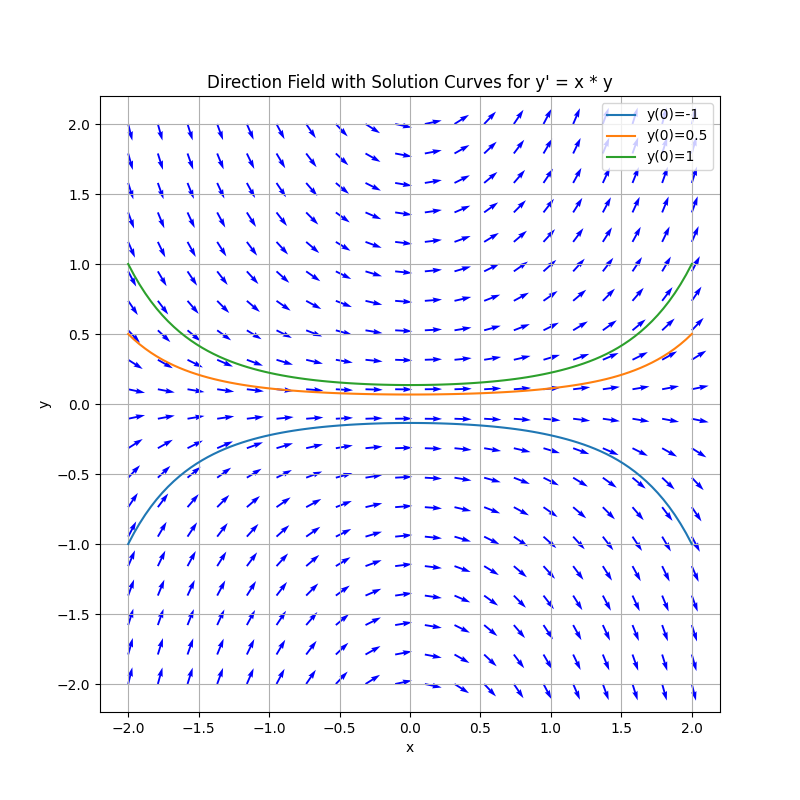
\includegraphics[width=\linewidth]{Graphs/direction_field.png}
  \end{enumerate}

  \subsection{Separable equations}

  \begin{enumerate}
    \item \textbf{Definition}: A first-order DE $y' = f(x,y)$ is called \hl{separable} if there are functions $g(x)$ and $h(y)$ such that \hl{$f(x,y) = g(x)h(y)$}, so a separable DE can be written
    \begin{center}
      \hl{$y' = g(x)h(y)$}
    \end{center}

    \item \textbf{Goal}: We want to find a method for solving separable DEs

    \item \textbf{Method}: We can solve a separable DE:
      \begin{center}
        $\frac{dy}{dx} = g(x)h(y)$
      \end{center}
    by separating variables.\\

    Dividing both sides by $h(y)$ gives 
      \begin{center}
        $\frac{1}{h(y)} \frac{dy}{dx} = g(x)$
      \end{center}

    Intergrating both sides gives:
      \begin{center}
        $\int \frac{1}{h(y)} = \int g(x) dx$ 
      \end{center}

    If we can find antiderivatives $H(y)$ for $\frac{1}{h(y)}$ and $G(x)$ for $g(x)$, then we have
      \begin{center}
        $H(y) = G(x) + C$ 
      \end{center}
  \end{enumerate}

  \section{Week3}
    \subsection{Modelling Population Growth}
      \begin{enumerate}
        \item \textbf{Constant Growth}: This occurs when the population $x$ increases at a constant rate. The DE is 
          \begin{center}
            $\frac{dx}{dt} = k$
          \end{center}
          where k is constant

        \item \textbf{Exponential Growth}: The exponential growth model assumes the growth rate is proportional to the size of the population.

        The general form of a DE modelling exponential growth is 
          \begin{center}
            $\frac{dx}{dt} = kx$
          \end{center}
          where k is constant

        \item \textbf{Logistic Growth}: Exponential growth is \hl{not} a realistic growth model for all values of $t$. \hl{A small animal population} with unlimited resources of food and space \hl{may show exponential growth initially}

        As the population gets larger there will be food shortages, overcrowding, and other factors that \hl{slow down the growth rate}.

        \hl{The growth rate k should decrease as the population x increases.}

        Since k is no longer constant, we write $k=g(x)$, so the DE becomes 
          \begin{center}
            $\frac{dx}{dt} = g(x)x$
          \end{center}

        A small population can growth exponentially, se we want \hl{$g(x) \approx k$} when \hl{$x \approx 0$}. But \hl{as x increases $g(x)$ should decrease.}

        The simplest formula with this behaviour is 
          \begin{center}
            $g(x) = k - ax$
          \end{center}

        So the DE becomes 
          \begin{center}
            $\frac{dx}{dt} = (k-ax)x$
          \end{center}

        We introduce a new constant $b = \frac{k}{a}$ so
          \begin{center}
            $(k-ax)x = ax (\frac{k}{a}-x) = ax(b-x)$
          \end{center}

        Let $\frac{b}{a} = b$, the logistic DE is then given by

          \begin{center}
            $\frac{dx}{dt} = ax(b-x)$
          \end{center}
      \end{enumerate}


\end{document}

